\section{Comparison of Performances}
\label{evaluation:comparison}

The hybrid DQM sampler from D-Wave solves the UCP with $14$ time instances a lot faster than the classical algorithm for solving MINLPs.
For problems with more time instances, this paper has no data from the classical solver.
Figure \ref{figure:evaluation.comparison.performance} shows the computing times needed to solve UCPs for the classical algorithm and the hybrid annealing-based algorithm for UCPs with up to $50$ time instances.
The line for the classical algorithm stops at $14$ time instances because this work does not test the classical algorithm on bigger problems.
Assuming that the classical algorithm has an exponential time complexity and the computation time continues like the graph in the figure, the hybrid annealing-based algorithm has a great advantage for bigger problems.

\begin{figure}
  \begin{subfigure}[b]{0.5 \textwidth}
    \centering
    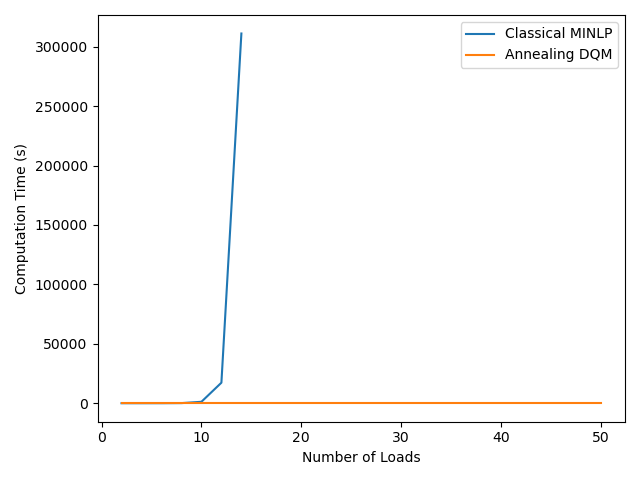
\includegraphics[width=\textwidth]{04_Validation/comparison_performance_c_dqm_p4.png}
    \caption{With up to $50$ Loads}
    \label{figure:evaluation.comparison.performance}
  \end{subfigure}
  \begin{subfigure}[b]{0.5 \textwidth}
    \centering
    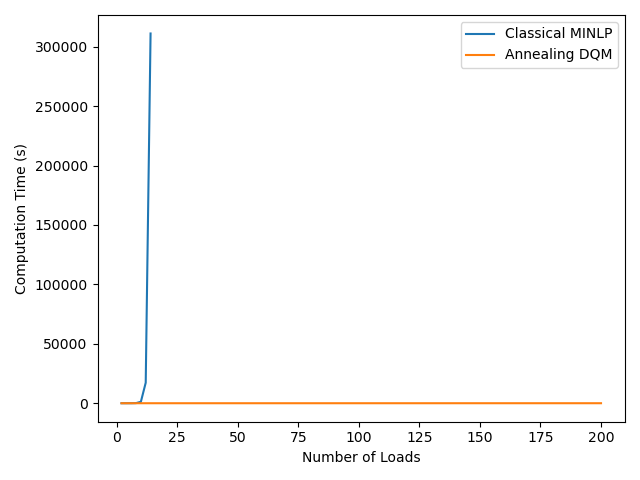
\includegraphics[width=\textwidth]{04_Validation/comparison_performance_c_dqm_p4_extended.png}
    \caption{With up to $200$ Loads}
    \label{figure:evaluation.comparison.performance.extended}
  \end{subfigure}
  \caption{Performance Comparison of Classical and Hybrid Annealing Algorithms}
\end{figure}

Although this improved computing time is astonishing, it is worthless if the hybrid annealing-based algorithm produces non-optimal results for the UCP problems.
For this reason, this work compares the solutions both algorithms produce based on the objective function $f(x)$ (\ref{formula:minlp.obj}).
The work computes the relative error of the solution of the hybrid annealing-based algorithm based on formula (\ref{formula:validation.relative.error}).
\begin{align}
  \label{formula:validation.relative.error}
  e_{\text{hybrid}}(x) = \quad \frac{f_{\text{hybrid}}(x) - f_{\text{classical}}(x)}{f_{\text{hybrid}}(x)}
\end{align}

Figure \ref{figure:evaluation.comparison.error} shows the error of the hybrid annealing-based algorithm the few experiments that this work runs using both the classical and the hybrid annealing-based algorithms.
While the error stays smaller than $0.5\%$ for these problems, it seems to grow exponentially.
There is no way to know how the solution error behaves for bigger problems without running the experiments using classical hardware.
Assuming that the error continues to grow exponentially with respect to the number of time instances in the UCP, the hybrid annealing-based algorithm produces worse solutions for larger UCPs.
It is crucial to highlight this trade-off in this work.

\begin{figure}
  \centering
  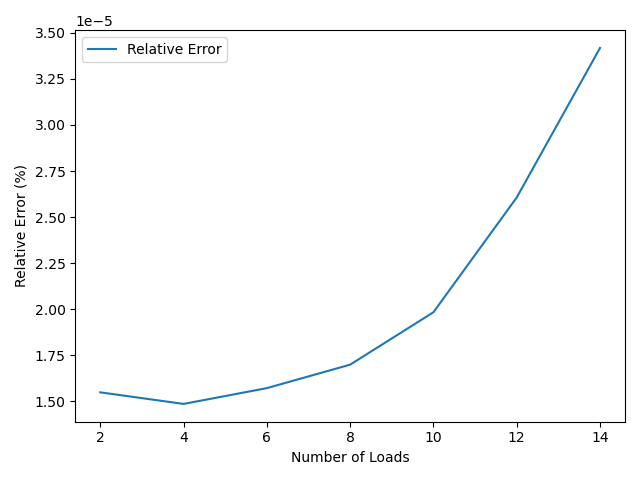
\includegraphics[width=0.7 \textwidth]{04_Validation/comparison_error_c_dqm_p4_.png}
  \caption{Relative Error of Hybrid Annealing Algorithm compared to Classical Algorithm}
  \label{figure:evaluation.comparison.error}
\end{figure}
